\chapter{Wdrożenie}
Wdrożenie aplikacji jest ostatnim etapem procesu tworzenia oprogramowania. Proces ten polega na przygotowaniu odpowiedniej konfiguracji środowiska i infrastruktury pod kątem skalowalności, bezpieczeństwa i ochrony przed awarią serwera. W projekcie wykorzystano technologię Docker oraz AWS, jednak ze względu na koszty AWS nie będzie wykorzystywany w dłuższym okresie czasu. Poniżej opisano szczegóły.

\section{Środowisko lokalne}
\textbf{Pobranie źródeł projektu~~} 
Pierwszym krokiem do wdrożenia aplikacji jest pobranie źródeł projekt. Aby to zrobić należy wpisać w terminal:
\begin{lstlisting}[basicstyle=\footnotesize\ttfamily]
git clone --recurse-submodules https://github.com/Bachelor-Thesis-Szewior-Joachim/deployment.git
\end{lstlisting}
Polecenie to utworzy lokalny klon zdalnego repozytorium kodu. Aby dało się to polecenie uruchomić, na komputerze użytkownika musi być zaistalowane narzędzie git.
Po pobarni źródeł można przejść do następnych kroków, tj.\ do zbudowania i uruchomienia odpowiednich dockerowych obrazów.\\[-10pt]

\noindent \textbf{Budowanie obrazów~~}
Aby uruchomić aplikację, należy zbudować obrazy dla 4 kontenerów:

\noindent
\begin{tabularx}{\linewidth}{XXXX}
$\bullet$ \texttt{frontend} &
$\bullet$  \texttt{backend} &
$\bullet$ \texttt{solana\_scripts} &
$\bullet$ \texttt{model\_server} 
\end{tabularx}\\[-10pt]

\noindent 
Obrazy można także pobrać z Docker Hub komendami:
\begin{lstlisting}[basicstyle=\footnotesize\ttfamily]
docker pull joaszek/bachelor-thesis:model_server_image
docker pull joaszek/bachelor-thesis:solana_scripts_image
docker pull joaszek/bachelor-thesis:backend_image
docker pull joaszek/bachelor-thesis:frontend_image
docker pull joaszek/bachelor-thesis:postgres_image
\end{lstlisting}

\noindent
Przykład zawartości pobranego pliku konfiguracyjnego:
\begin{lstlisting}[basicstyle=\footnotesize\ttfamily,tabsize=2]
version: "3.8"

services:
  postgres:
    image: postgres:16
    container_name: postgres_db
    environment:
      POSTGRES_USER: myuser
      POSTGRES_PASSWORD: mypassword
      POSTGRES_DB: mydatabase
    volumes:
      - ./backup.sql:/docker-entrypoint-initdb.d/backup.sql
      - backend_pg_data:/var/lib/postgresql/data
    ports:
      - "5432:5432"
    networks:
      - my_network

  pgadmin:
    image: dpage/pgadmin4
    container_name: pgadmin
    environment:
      PGADMIN_DEFAULT_EMAIL: admin@admin.com
      PGADMIN_DEFAULT_PASSWORD: admin
    ports:
      - "5050:80"
    depends_on:
      - postgres
    networks:
      - my_network

  backend_app:
    image: backend_image
    container_name: spring_app
    privileged: true
    volumes:
      - ./backend:/app
      - /var/run/docker.sock:/var/run/docker.sock
    environment:
      SPRING_DATASOURCE_URL: jdbc:postgresql://postgres:5432/mydatabase
      SPRING_DATASOURCE_USERNAME: myuser
      SPRING_DATASOURCE_PASSWORD: mypassword
      SPRING_JPA_HIBERNATE_DDL_AUTO: update
      SPRING_JPA_SHOW_SQL: "true"
      SPRING_JPA_PROPERTIES_HIBERNATE_DIALECT: org.hibernate.dialect.PostgreSQLDialect
      COINMARKETCAP_API_URL: d42f0690-3288-4f73-8230-da9ac5135859
    ports:
      - "8080:8080"
    depends_on:
      - postgres
    networks:
      - my_network

  solana_scripts_service:
    image: solana_scripts_image
    container_name: solana_scripts_service
    volumes:
      - ./backend/src/main/java/org/example/backend/client/client/service/solanaScripts:/app
    working_dir: /app
    ports:
      - "3001:3001"
    command: ["npm", "start"]
    networks:
      - my_network

  model_server:
    image: model_server
    container_name: model_server
    ports:
      - "5000:5000"
    networks:
      - my_network
    volumes:
      - ./models:/models

  frontend_app:
    image: frontend_image
    container_name: frontend_app
    volumes:
      - ./frontend:/usr/app
    ports:
      - "3000:3000"
    command: ["npm", "start"]
    networks:
      - my_network

volumes:
  backend_pg_data:

networks:
  my_network:
    driver: bridge
\end{lstlisting}

Następnie należy uruchomić komendę \texttt{docker compose up} w folderze, w którym jest \texttt{docker-compose.yml} aby postawić aplikację na swoim komputerze.

\section{Środowisko AWS}
\textbf{Serwisy~~}
Aplikacja została wdrożona w środowisku AWS z wykorzystaniem usługi ECS (ang.~\emph{Elastic Container Service}) w trybie Fargate. Skonfigurowano następujące serwisy:
\begin{itemize}
    \item \textbf{Postgres}:
    \begin{itemize}
        \item Obraz: \url{503561436372.dkr.ecr.eu-north-1.amazonaws.com/bachelor/deployment:postgres_custom}
        \item Port: \texttt{5432}
        \item Zmienne środowiskowe:
        \begin{itemize}
            \item \texttt{POSTGRES\_USER: myuser}
            \item \texttt{POSTGRES\_PASSWORD: mypassword}
            \item \texttt{POSTGRES\_DB: mydatabase}
        \end{itemize}
    \end{itemize}
    \item \textbf{PgAdmin}:
    \begin{itemize}
        \item Obraz: \texttt{dpage/pgadmin4}
        \item Port: \texttt{5050}
        \item Zmienne środowiskowe:
        \begin{itemize}
            \item \texttt{PGADMIN\_DEFAULT\_EMAIL: admin@admin.com}
            \item \texttt{PGADMIN\_DEFAULT\_PASSWORD: admin}
        \end{itemize}
    \end{itemize}
    \item \textbf{Backend App}:
    \begin{itemize}
        \item Obraz: \url{503561436372.dkr.ecr.eu-north-1.amazonaws.com/bachelor/deployment:backend_image_latest}
        \item Port: \texttt{8080}
        \item Zmienne środowiskowe:
        \begin{itemize}
            \item \texttt{SPRING\_JPA\_SHOW\_SQL: true}
            \item \texttt{SPRING\_DATASOURCE\_URL: jdbc:postgresql://postgres:5432/mydatabase}
            \item \texttt{SPRING\_DATASOURCE\_PASSWORD: mypassword}
            \item \texttt{SPRING\_JPA\_HIBERNATE\_DDL\_AUTO: update}
            \item \texttt{SPRING\_DATASOURCE\_USERNAME: myuser}
            \item \texttt{COINMARKETCAP\_API\_URL: ...}
        \end{itemize}
    \end{itemize}
    \item \textbf{Solana Scripts Service}:
    \begin{itemize}
        \item Obraz: \url{503561436372.dkr.ecr.eu-north-1.amazonaws.com/bachelor/deployment:solana_scripts_image_latest}
        \item Port: \texttt{3001}
        \item Polecenie startowe: \texttt{npm start}
    \end{itemize}
    \item \textbf{Model Server}:
    \begin{itemize}
        \item Obraz: \url{503561436372.dkr.ecr.eu-north-1.amazonaws.com/bachelor/deployment:model_server_image_latest}
        \item Port: \texttt{5000}
    \end{itemize}
    \item \textbf{Frontend App}:
    \begin{itemize}
        \item Obraz: \url{503561436372.dkr.ecr.eu-north-1.amazonaws.com/bachelor/deployment:frontend_image_latest}
        \item Port: \texttt{3000}
        \item Polecenie startowe: \texttt{npm start}
    \end{itemize}
\end{itemize}

\textbf{Skalowanie i infrastruktura~~}
W ramach infrastruktury AWS zostały skonfigurowane:
\begin{itemize}
    \item Dwa subnety:
    \begin{itemize}
        \item \textbf{Publiczny subnet} do komunikacji z internetem.
        \item \textbf{Prywatny subnet} dla wewnętrznych usług, takich jak baza danych.
    \end{itemize}
    \item Specjalna sieć VPC (\textit{Virtual Private Cloud}) dedykowana dla tej aplikacji.
    \item Security Group z odpowiednimi regułami dostępu, zezwalającymi na ruch przychodzący i~wychodzący na portach używanych przez aplikację (3000, 8080, 5432, 5050, 5000).
    \item Rola IAM o nazwie \texttt{ECS\_Role}, która umożliwia ECS dostęp do obrazów w ECR i logowanie do CloudWatch.
    \item Load Balancer, który rozdziela ruch do aplikacji i zapewnia wysoką dostępność.
\end{itemize}


\section{Użytkowanie aplikacji}
\subsection{Logowanie i rejestracja}
Aby móc skorzystać z aplikacji potrzebne jest konto na stronie. Strona startowa aplikacji jest stroną do logowania. Pokazano ją na rysunku~\ref{fig:Logowanie}a. Jeżeli użytkownik nie ma konta, należy kliknąć w przycisk \texttt{Sign up}, aby się zarejestrować. 
% TO DO: do każdego rysunku trzeba jawnie się odnieść. Pisałem o tym w szablonie pracy !!!!!
%        prosze odpowiednio przeradagować tekst poniżej
%        Czy da się jeszcze bardziej zawęzić okna przed zrobieniem zrzutów z ekranu? Jeśli tak, to proszę zrobić nowe zrzuty.
\subsection{Strona główna}
Po zalogowaniu  użytkownik zostanie przeniesiony na główną stronę o wyglądzie pokazanym na rysunku na rysunku~\ref{fig:Logowanie}b. 
Na górze każdej strony będzie pasek z zakładkami: \texttt{Blockchain}, \texttt{Tokens}, \texttt{Cryptocurrency}, \texttt{Resources}.
\begin{figure}[htb]
    \centering
		\begin{tabular}{l}
    a) \\ \vtop{\vskip-2ex\hbox{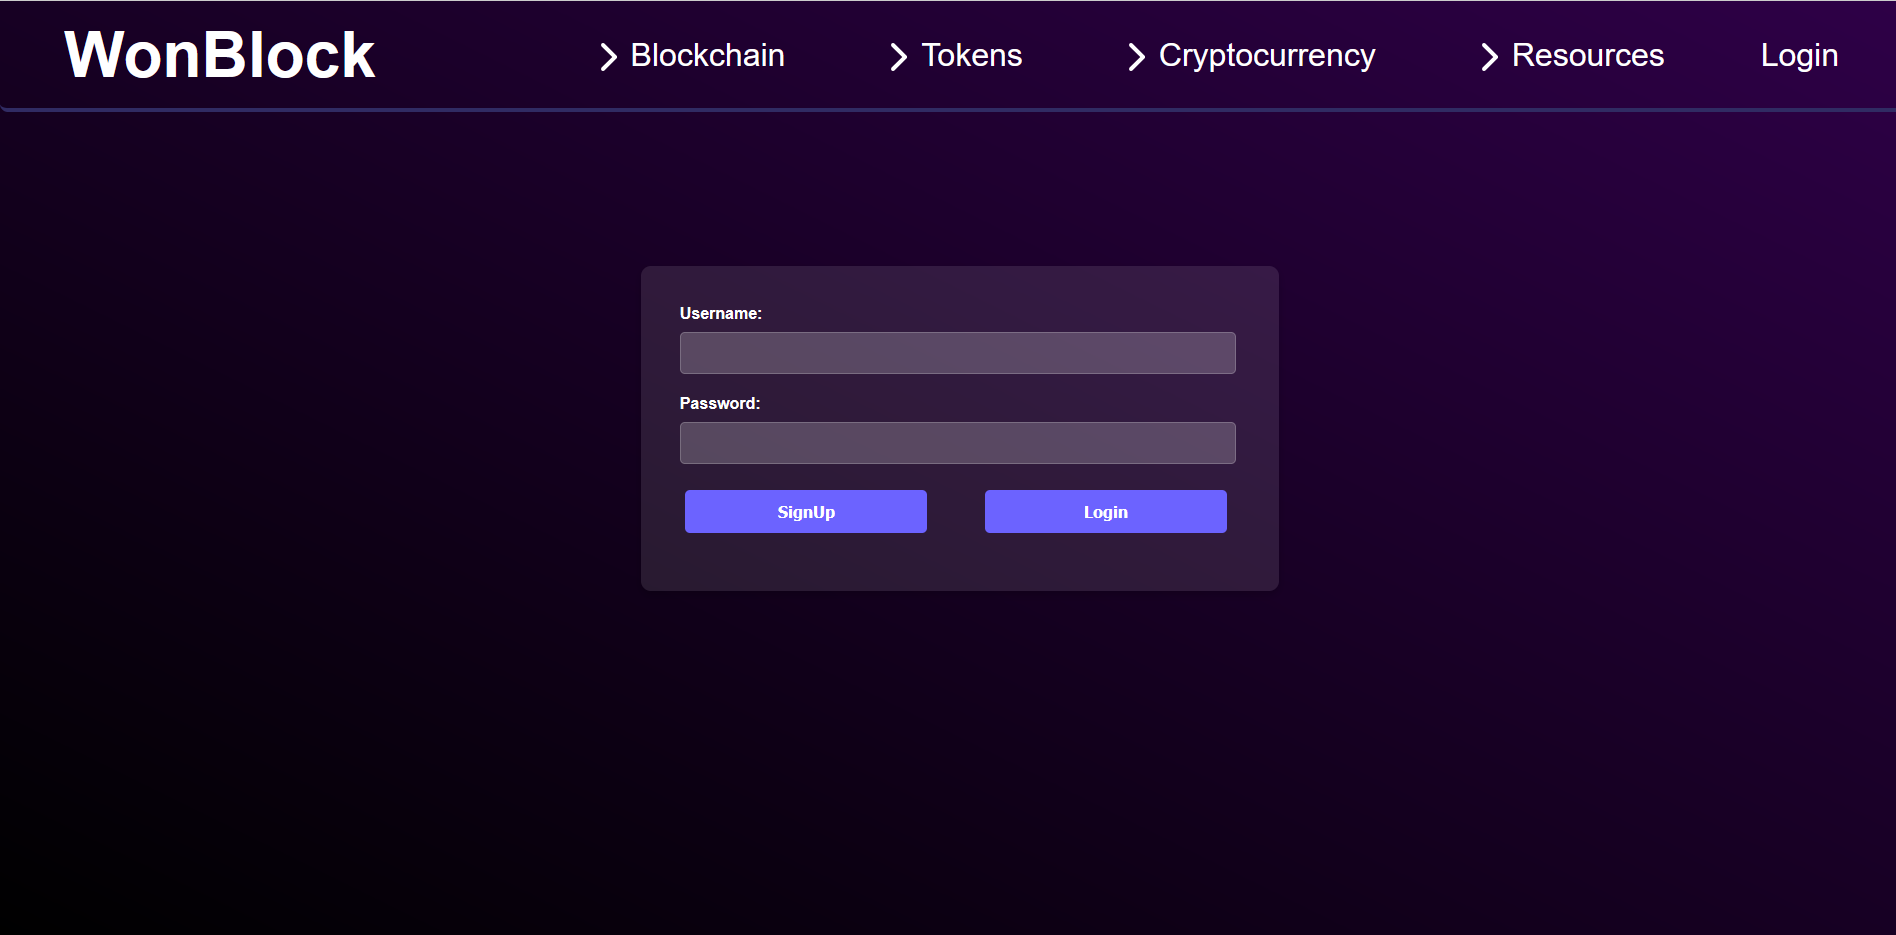
\includegraphics[width=0.9\linewidth]{./instrukcja/Login.png}}}\\ 
		b) \\ \vtop{\vskip-2ex\hbox{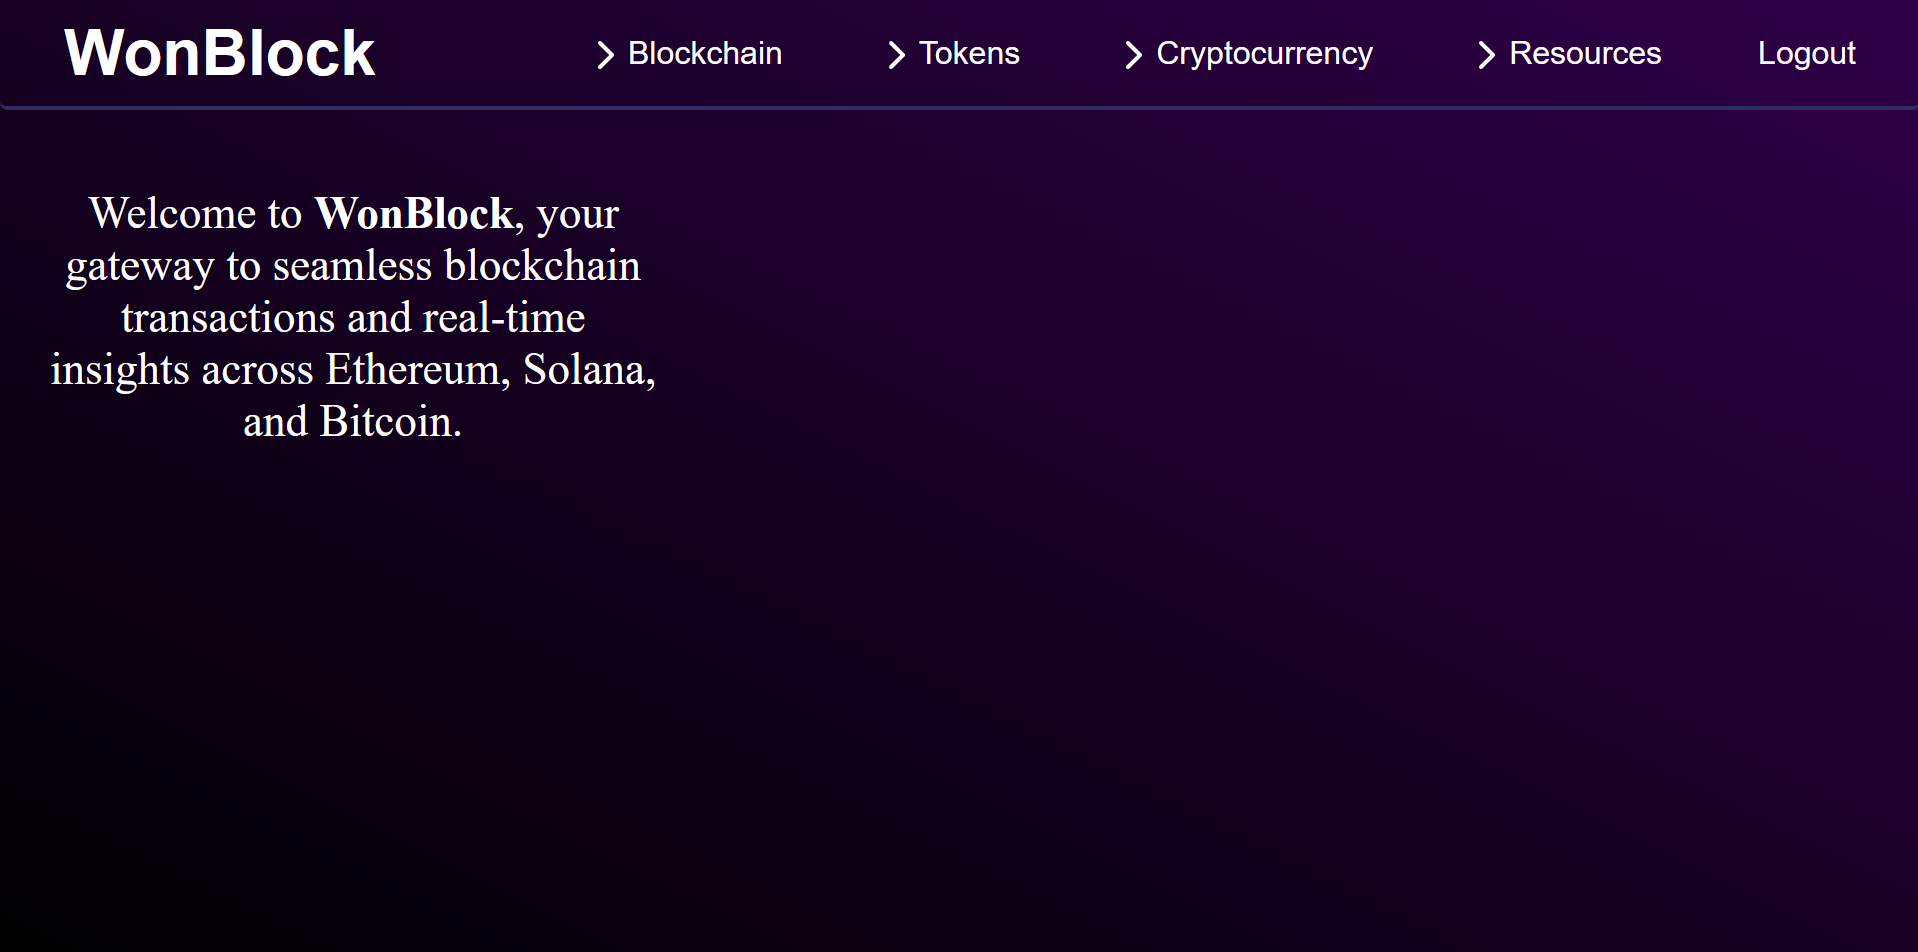
\includegraphics[width=0.9\linewidth]{./instrukcja/mainpage.png}}}
		\end{tabular}
    \caption{Interfejs użytkownika: a) logowanie, b) strona główna}
    \label{fig:Logowanie}
\end{figure}

\subsubsection{Zakładka \texttt{Blockchain}}
Zakładka ta daje dostęp do opcji: \texttt{Accounts}, \texttt{View Blocks}, \texttt{Transactions}.

Opcja \texttt{Accounts} pozwala na wyszukania konta. Aby to zrobić należy wpisać adres oraz wybrać blockchain, z którego pochodzi dany adres (patrz rysunek~\ref{fig:Konta}a). Po tej akcji system automatycznie przeniesie użytkownika na nową stronę z danymi konta (patrz rysunek~\ref{fig:Konta}b). Sprawdzanie bloków w opcji \texttt{View Blocks} oraz transakcji w opcji \texttt{Transactions} działa analogicznie.
\begin{figure}[htb]
    \centering
		\begin{tabular}{l}
		a) \\ \vtop{\vskip-2ex\hbox{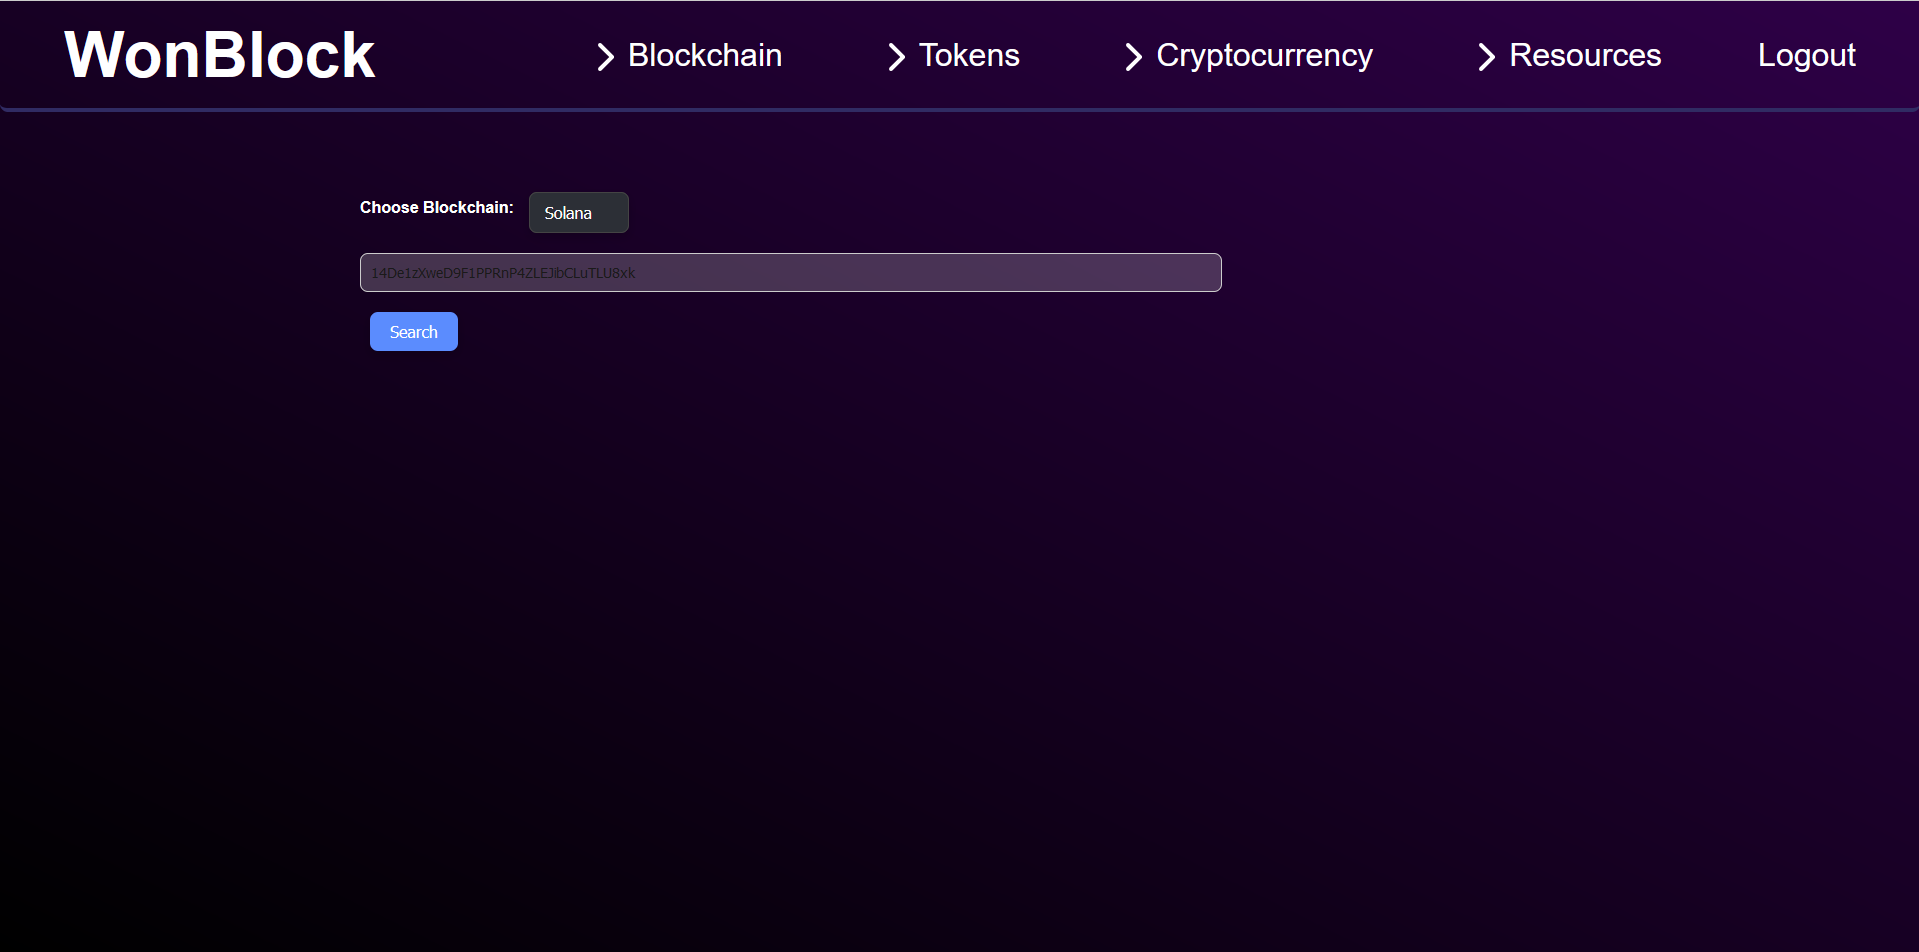
\includegraphics[width=0.9\linewidth]{./instrukcja/Check_account.png}}} \\
		b) \\ \vtop{\vskip-2ex\hbox{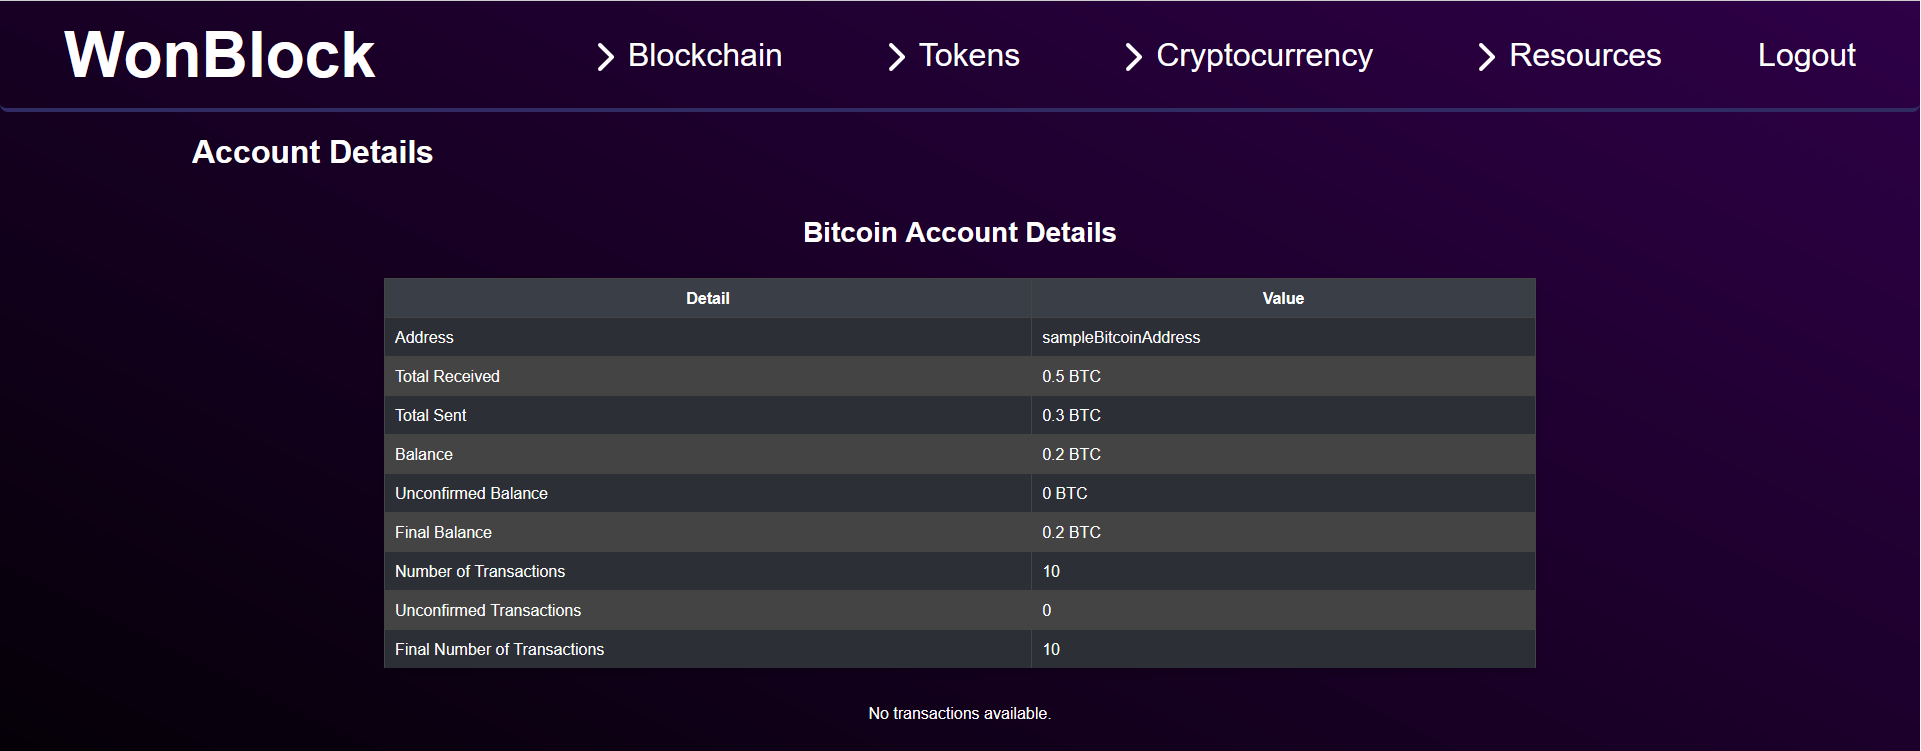
\includegraphics[width=0.9\linewidth]{./instrukcja/Account_details.png}}}
		\end{tabular}
    \caption{Interfejs użytkownika: znajdź konto, d) dane konta}
    \label{fig:Konta}
\end{figure}

\subsubsection{Zakładka \texttt{Tokens}}
Zakładka ta oferuje dwie opcje: \texttt{Collection} oraz \texttt{General NFT statistics}. Jeśli użytkownik wybierze, opcję \texttt{Collection}, to zostanie przeniesiony na stronę z listami kolekcji zaprezentowaną na rysunku~\ref{fig:Collections}a.
Drugą opcją do wyboru jest \texttt{General NFT statistics}. Po jej wybraniu użytkownik zostanie przeniesiony na stronę jak rysunku~\ref{fig:Collections}b. Na tej stronie użytkownik może szukać tokenów po atrybutach: Kontrakt, Identyfikator, Nazwa, Kolekcja.
\begin{figure}[htb]
    \centering
		\begin{tabular}{l}
    a) \\ \vtop{\vskip-2ex\hbox{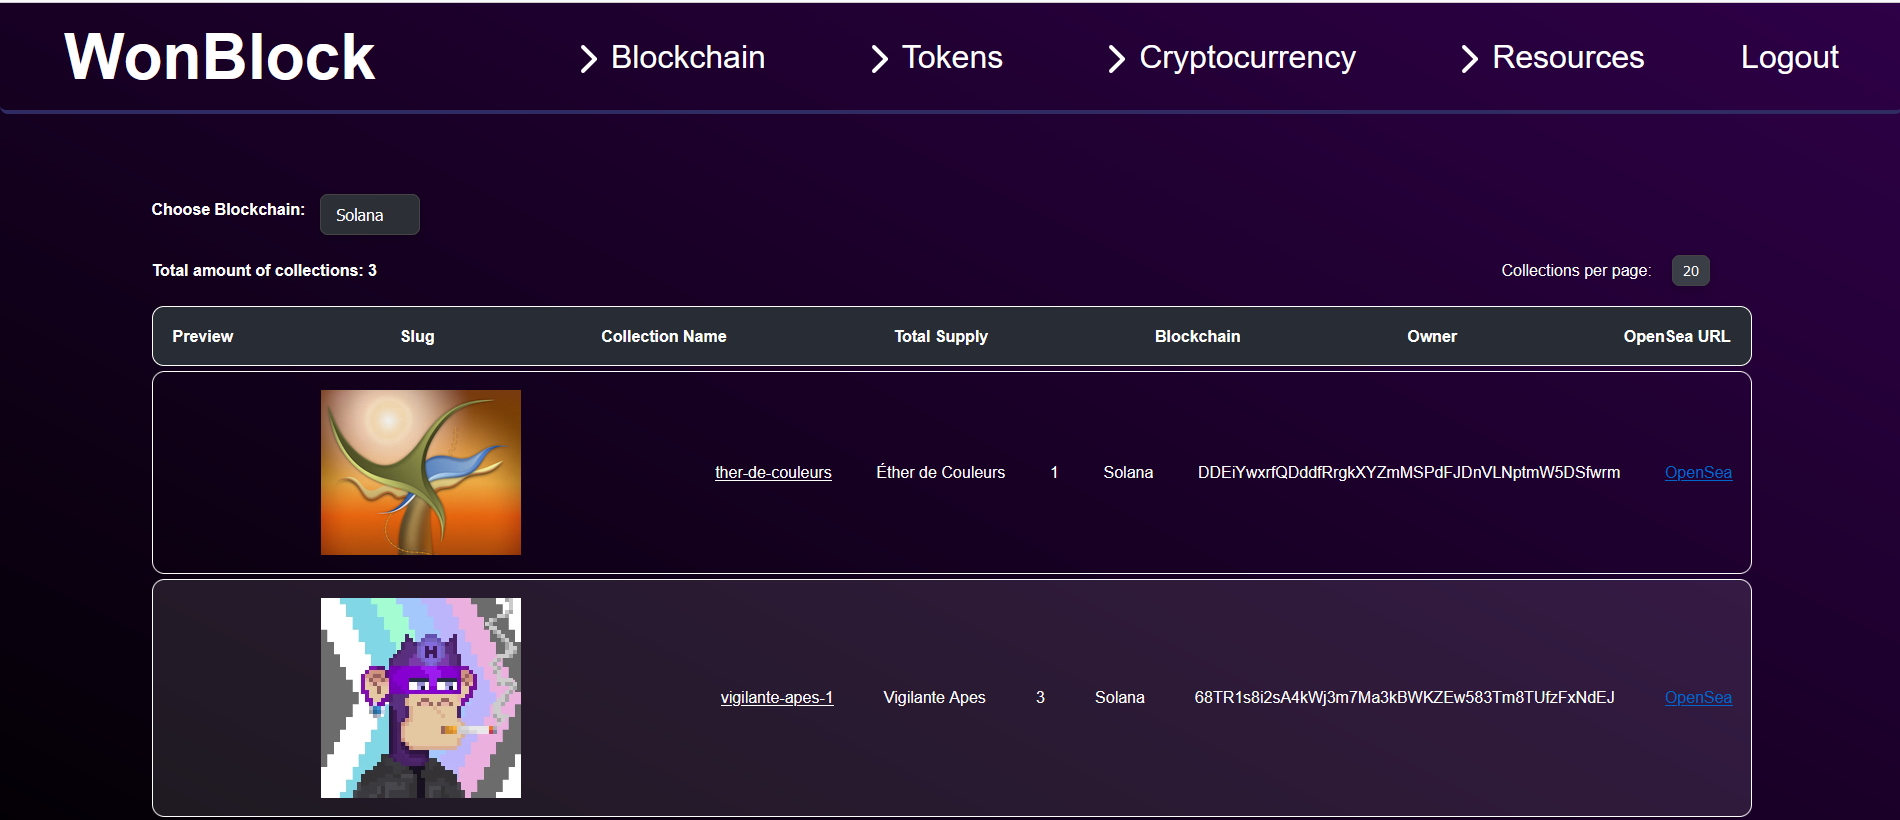
\includegraphics[width=0.9\linewidth]{./instrukcja/Collections.png}}} \\
		b) \\ \vtop{\vskip-2ex\hbox{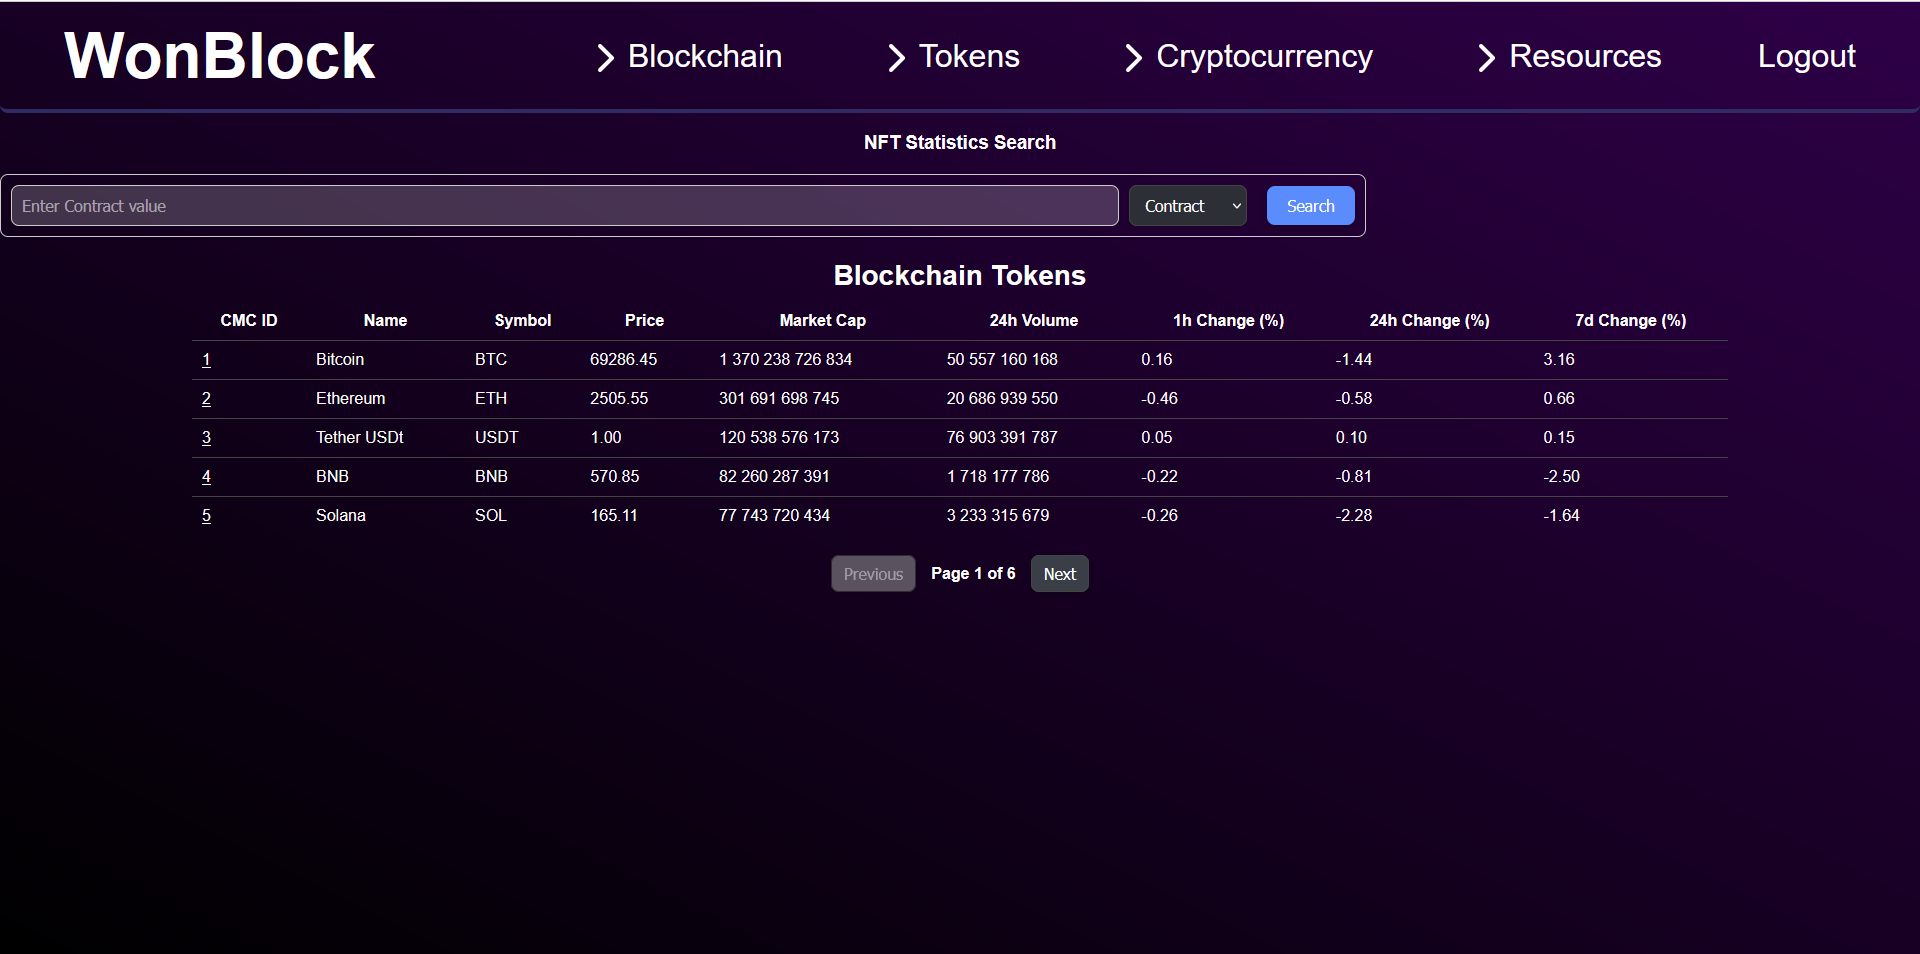
\includegraphics[width=0.9\linewidth]{./instrukcja/Tokens.png}}}
		\end{tabular}
    \caption{Zakładka \texttt{Tokens}: a) \texttt{Collection}, b) \texttt{General NFT statistics}}
    \label{fig:Collections}
\end{figure}

\subsection{Zakładka \texttt{Cryptocurrency}}
Na zakładce \texttt{Cryptocurrency} użytkownik może wybrać jedną z opcji: \texttt{Ranking}, \texttt{Categories}, \texttt{Global market}, \texttt{Historical data}, \texttt{Gainers \& Losers}.

Opcja \texttt{Ranking} pokaże listę tokenów jak na rysunku~\ref{fig:Cryptocurrency}a. Opcja \texttt{Categories} pozwala na zobaczenie listy kategorii. Opcja \texttt{Global market} oraz \texttt{Gainers and Losers} pokazuje wykresy na temat globalnych rynków oraz na statystykę \texttt{Gainers and Losers} odpowiednio. Opcja \texttt{Historical Data} pokaże kalendarz, z którego można wybrać dowolną datę sprzed dwóch lat, aby zobaczyć stan rankingu na dany dzień (patrz rysunek~\ref{fig:Cryptocurrency}b)
\begin{figure}[htb]
    \centering
		\begin{tabular}{l}
    a) \\ \vtop{\vskip-2ex\hbox{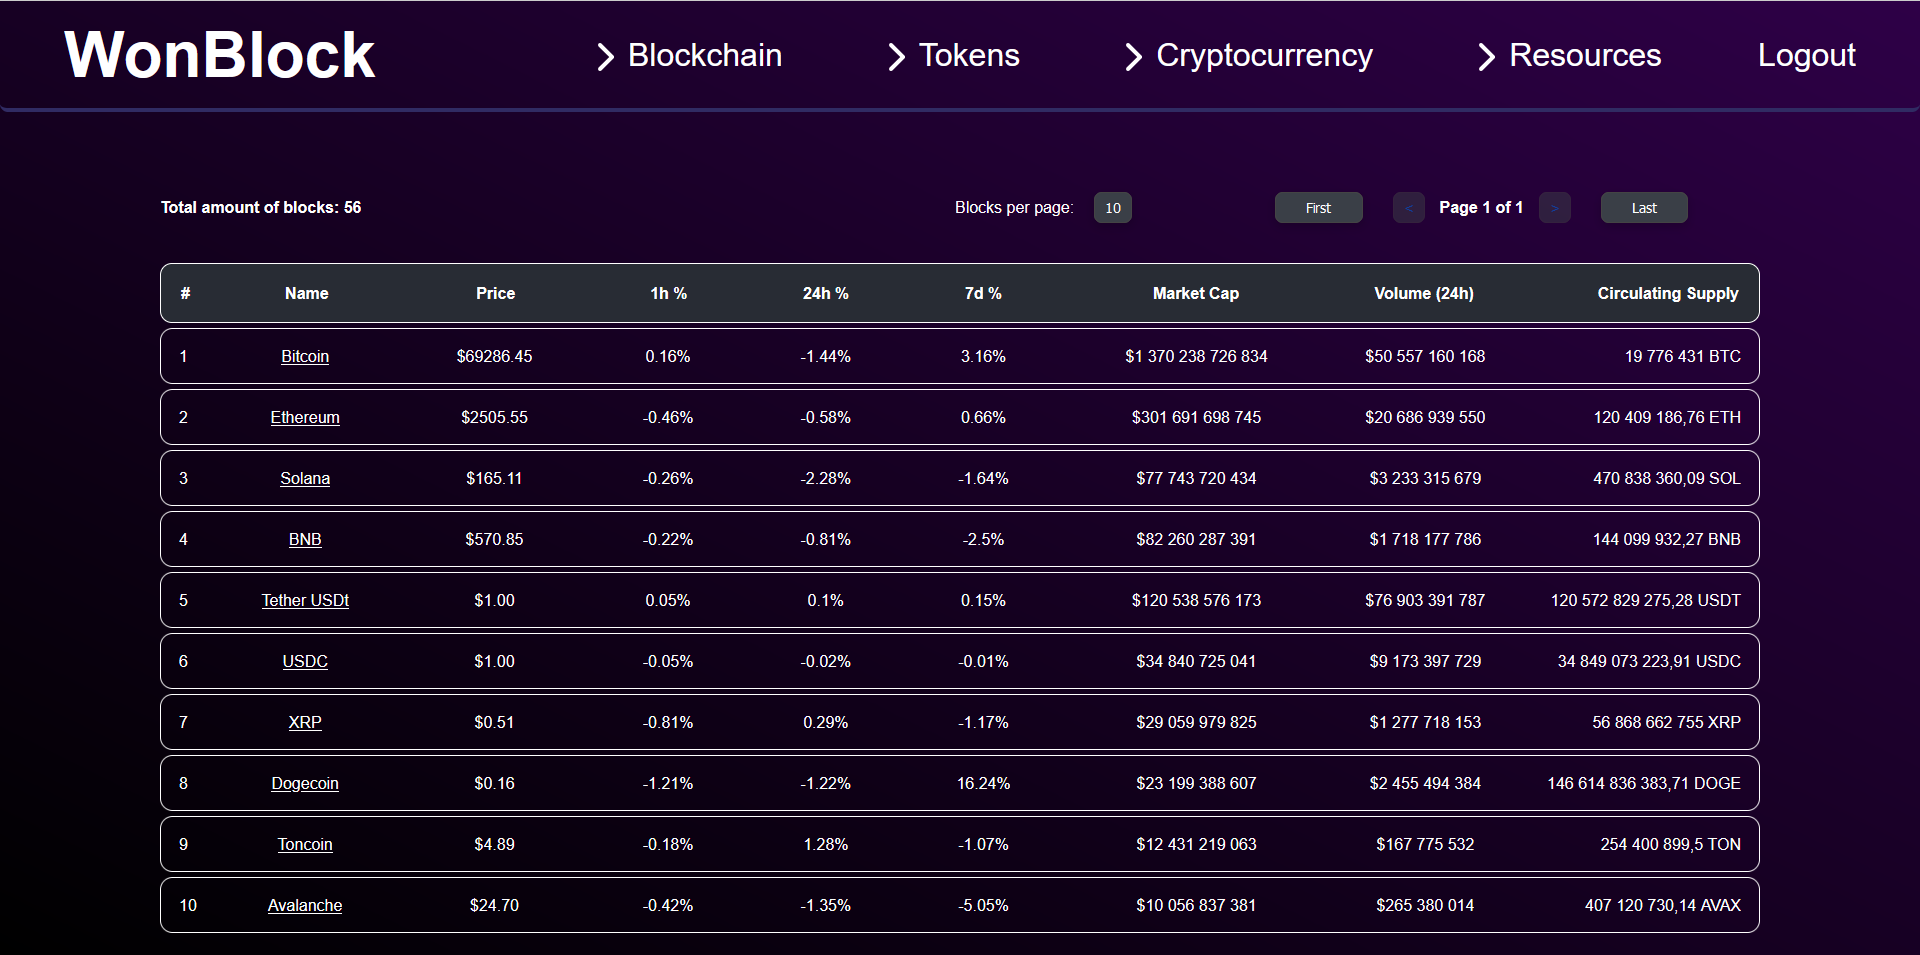
\includegraphics[width=0.9\linewidth]{./instrukcja/Ranking.png}}} \\
		b) \\ \vtop{\vskip-2ex\hbox{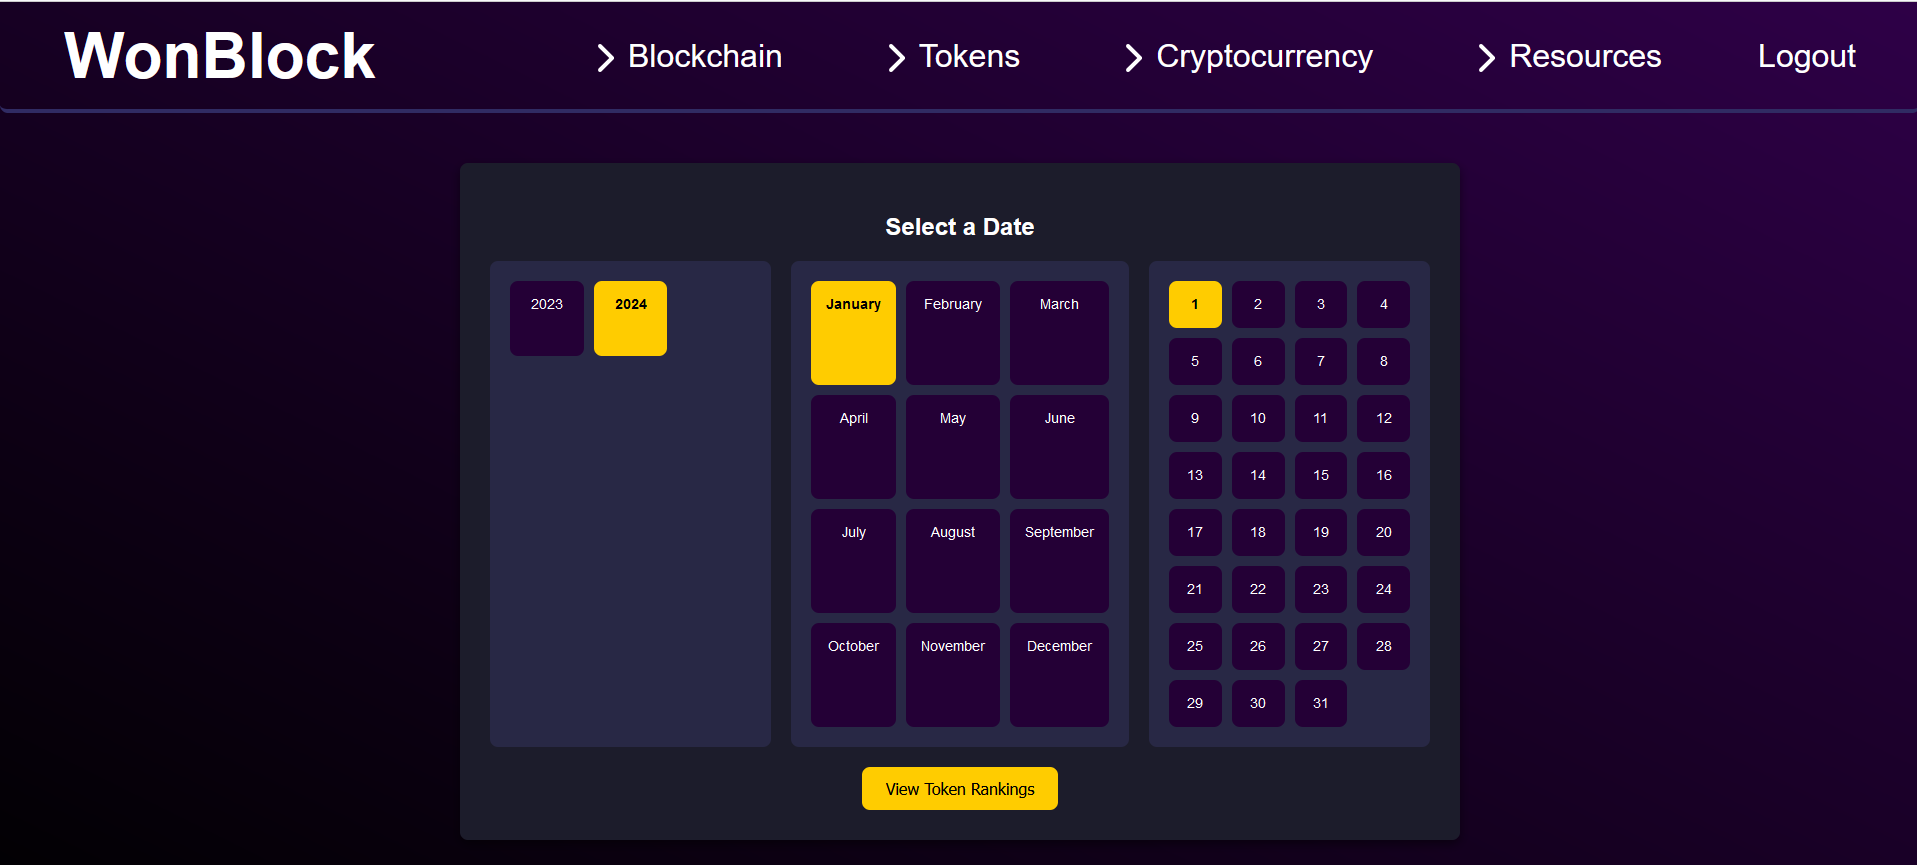
\includegraphics[width=0.9\linewidth]{./instrukcja/HistoricalData.png}}}
\end{tabular}
    \caption{Zakładka \texttt{Cryptocurrency}: a) \texttt{Ranking}, b) \texttt{Historical data}}
    \label{fig:Cryptocurrency}
\end{figure}

\newpage
\subsection{Zakładka \texttt{Resources}}
Zakładka \texttt{Resources} pozwala użytkownikowi na uruchomienie opcji: \texttt{Converter}, \texttt{Directory}, \texttt{News}, \texttt{Simulate Transaction}, \texttt{Predict Prices}.

Opcja \texttt{Converter} pozwala na przekonwertowanie walut i kryptowalut na interfejsie jak na rysunku~\ref{fig:Resources}a.
Opcja \texttt{Directory} zawiera różne źródła, z których użytkownik może się uczyć na temat technologii blockchain.
Opcja \texttt{News} zawiera najnowsze informacje ze świata na temat różnych blockchainów.
Opcja \texttt{Simulate Transaction} pozwala użytkowniki na wpisanie tekstu i zasymulowanie transakcji na interfejsie jak na rysunku~\ref{fig:Resources}b.
\begin{figure}[htb]
    \centering
		\begin{tabular}{l}
    a) \\ \vtop{\vskip-2ex\hbox{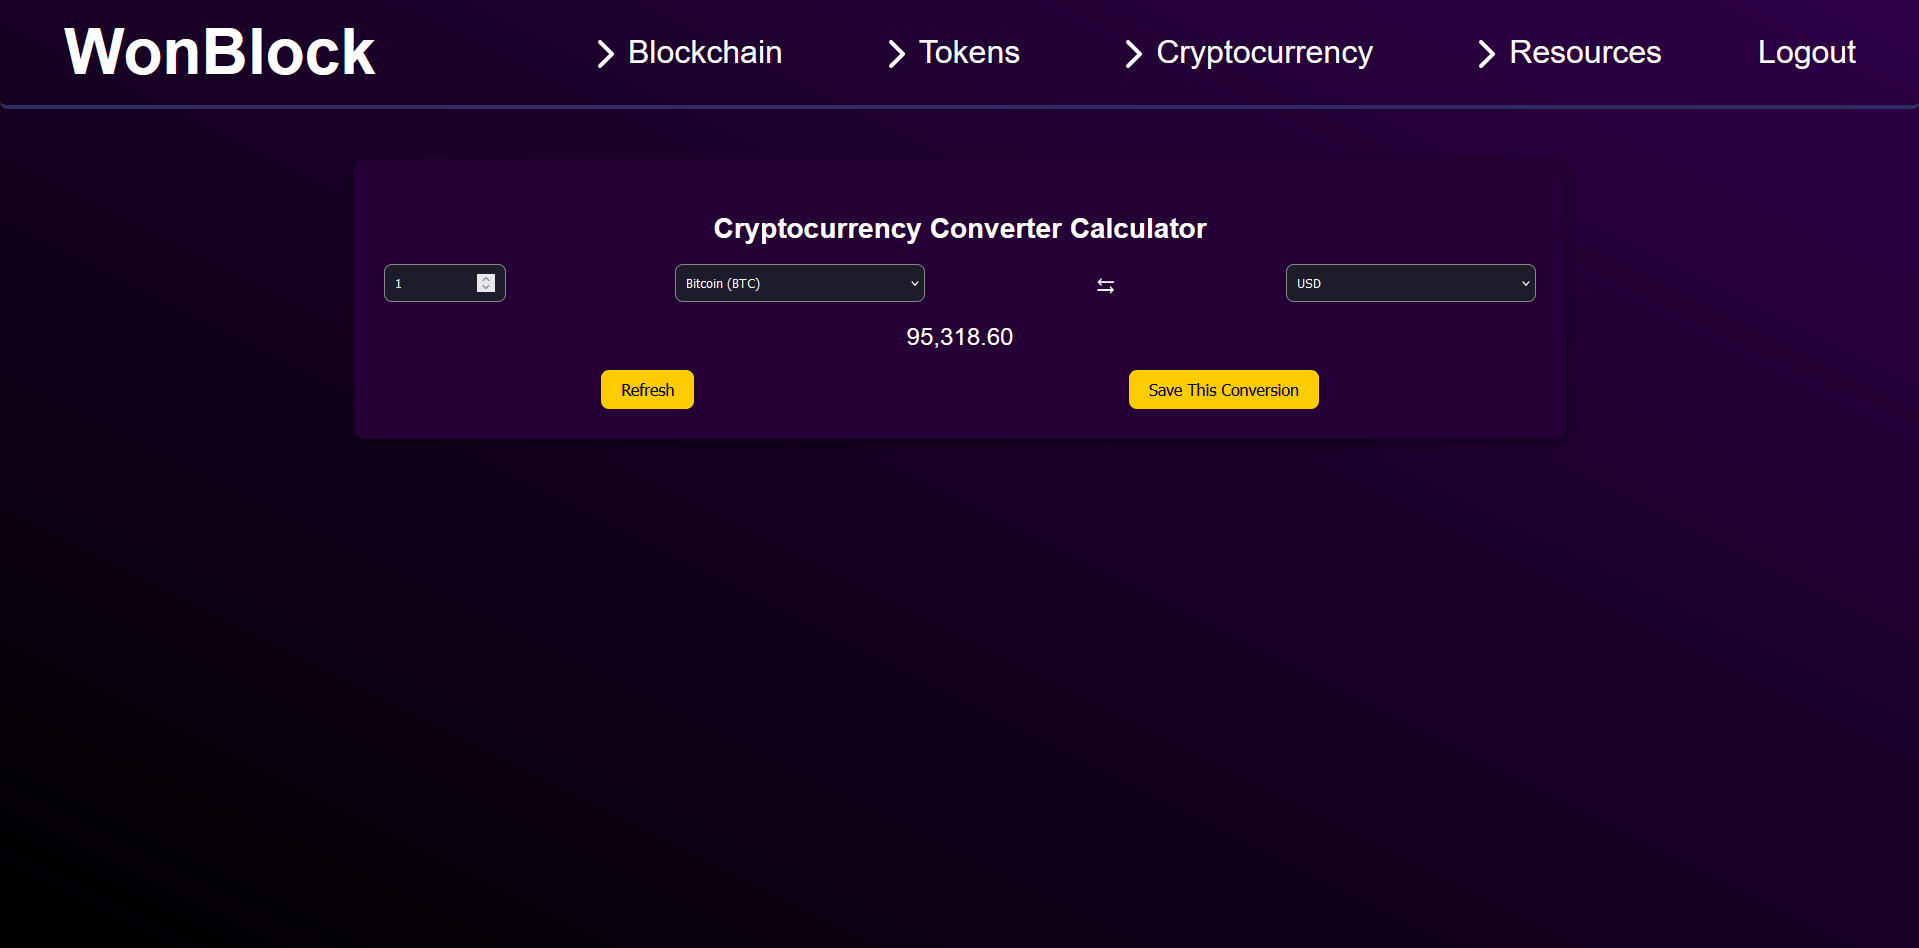
\includegraphics[width=0.8\linewidth]{./instrukcja/Converter.png}}} \\
		b) \\ \vtop{\vskip-2ex\hbox{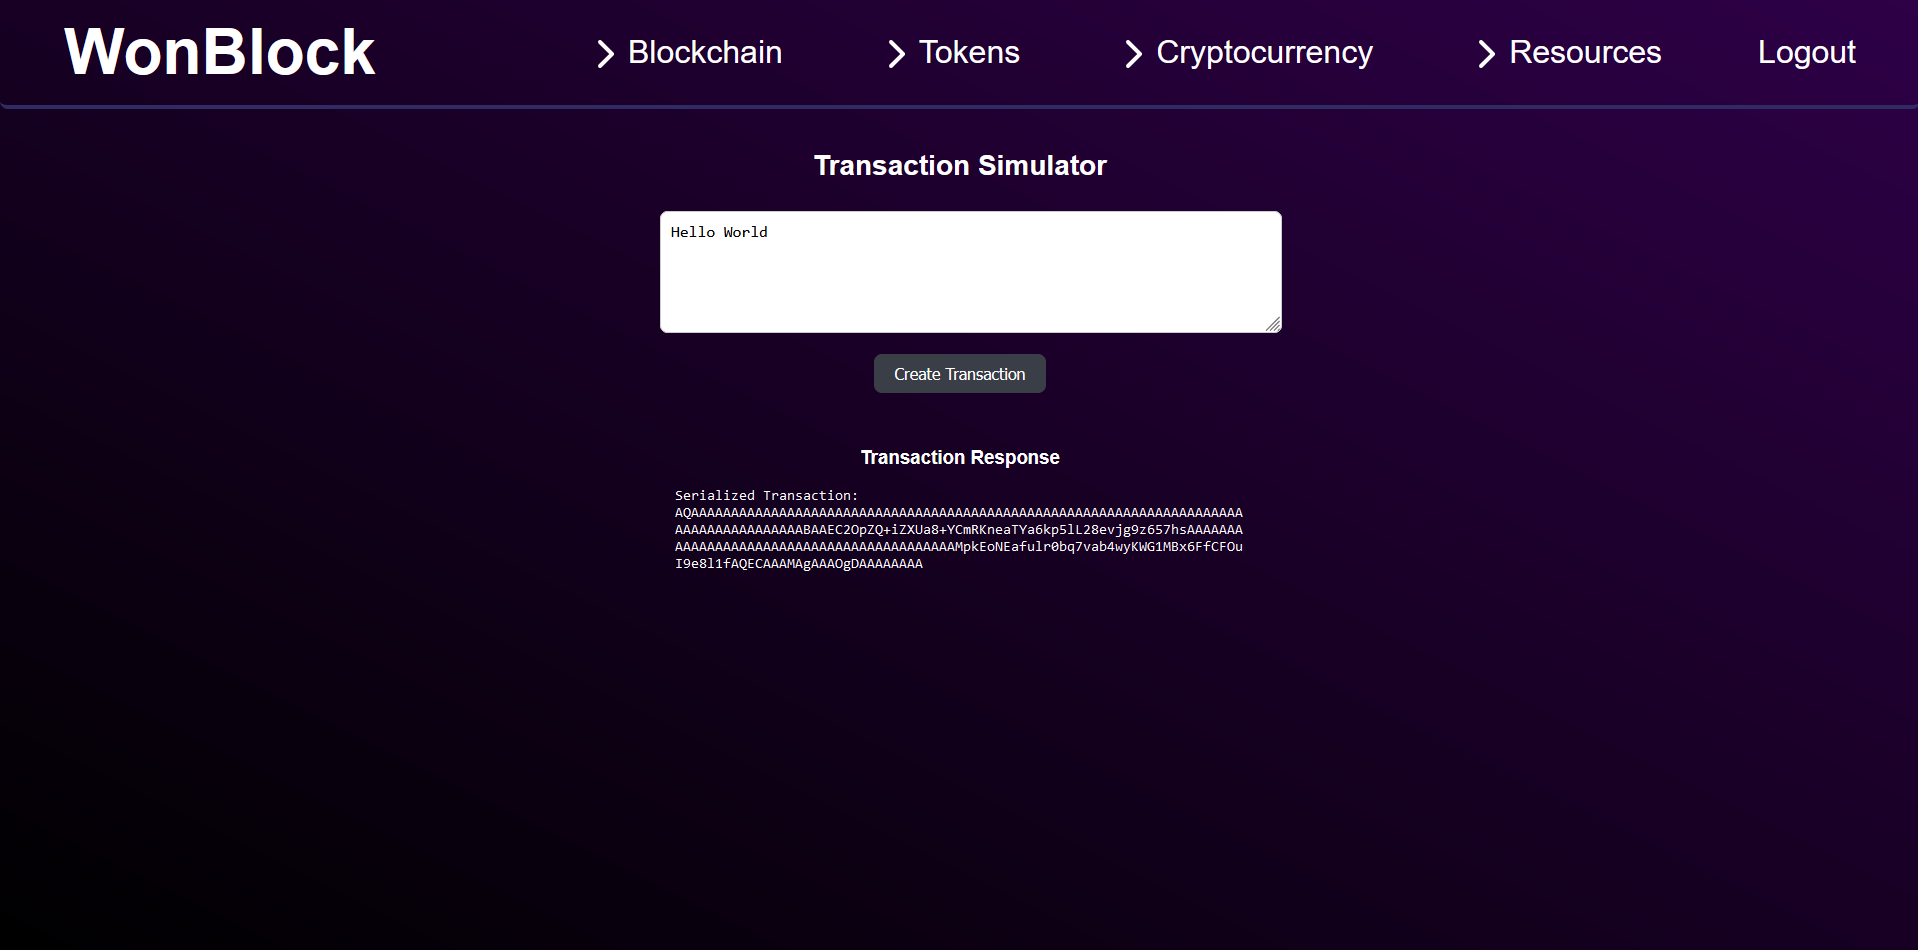
\includegraphics[width=0.8\linewidth]{./instrukcja/SimulateTransaction.png}}}
\end{tabular}
    \caption{Zakładka \texttt{Resources}: a) \texttt{Converter}, b) \texttt{Simulate Transaction}}
    \label{fig:Resources}
\end{figure}

\newpage
\subsubsection{Przewidywanie cen}
Opcja \texttt{Predict prices} pozwala użytkowniki na poznanie przewidywanych wartości dla kryptowalut Bitcoin, Ether oraz Sol. Widok oferowany użytkownikowi w tym przypadku jest jak na rysunku~\ref{fig:Przewidywanie cen}.
\begin{figure}[htb]
    \centering
    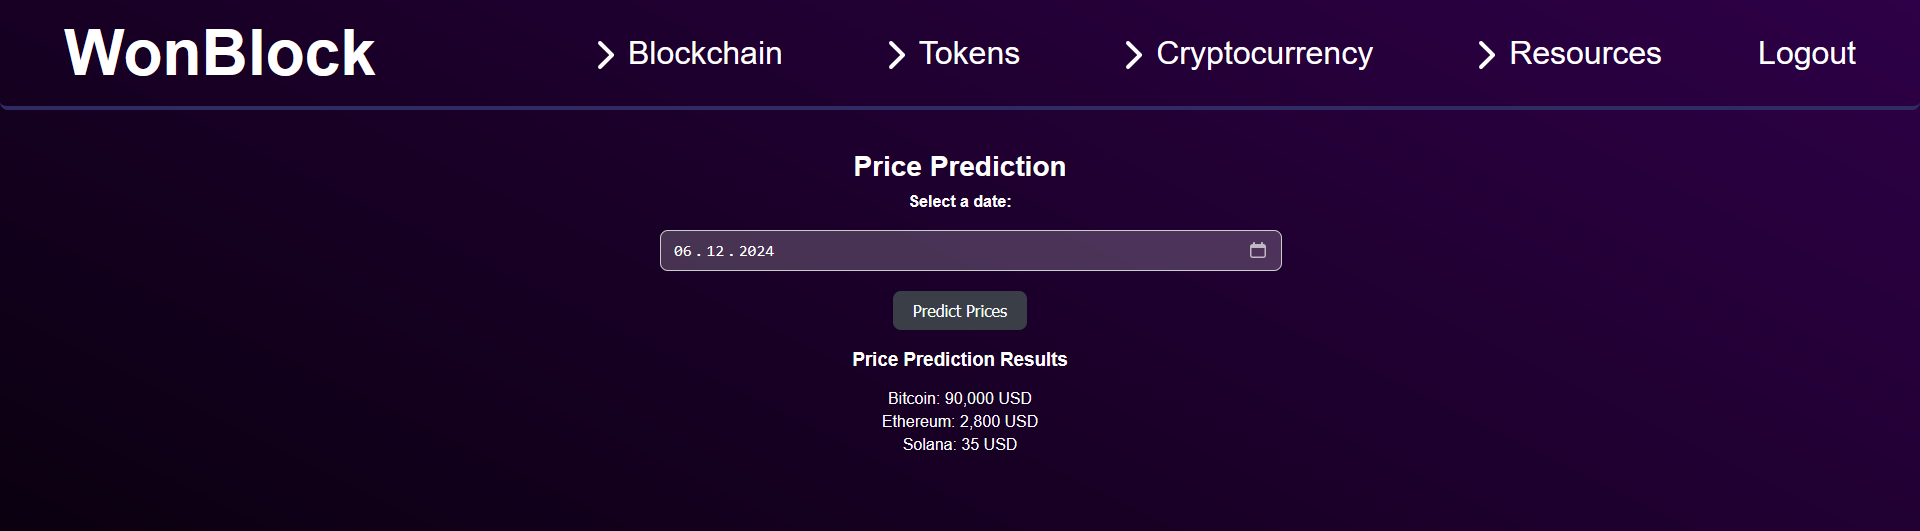
\includegraphics[width=0.8\linewidth]{./instrukcja/PredictPrices.png}
    \caption{Przewidywanie cen}
    \label{fig:Przewidywanie cen}
\end{figure}